\chapter{Element Parameter Groups}
\label{c:ele.groups}

Generally, element parameters are grouped into ``\vn{element} \vn{parameter} \vn{group}'' 
types which is discussed in \sref{c:ele}.

Element parameter groups inherit from the abstract type \vn{EleParameterGroup} which
in turn inherits from \vn{BaseEleParameterGroup}. Some
parameter groups have sub-group components. 
These sub-groups also inherit from \vn{BaseEleParameterGroup}:
\begin{example}
  abstract type BaseEleParameterGroup end
  abstract type EleParameterGroup <: BaseEleParameterGroup end
  abstract type EleParameterSubGroup <: BaseEleParameterGroup end
\end{example}

All parameter groups have associated docstrings that can be accessed when using the REPL.

The parmeters groups are:
\begin{table}[htb]
\centering
{\tt
\begin{tabular}{llll} \toprule
  {\it Group}        & {\it Section}         & {\it Group}      & {\it Section}         \\ \midrule
 AlignmentGroup      & \sref{s:align.g}      & ApertureGroup    & \sref{s:apert.g}      \\
 BMultipoleGroup     & \sref{s:bmult.g}      & BeamBeamGroup    & \sref{s:bb.g}         \\
 BendGroup           & \sref{s:bend.g}       & EMultipoleGroup  & \sref{s:emult.g}      \\
 FloorPositionGroup  & \sref{s:floor.g}      & GirderGroup      & \sref{s:girder.g}     \\
 InitParticleGroup   & \sref{s:initp.g}      & LCavityGroup     & \sref{s:lcav.g}       \\
 LengthGroup         & \sref{s:length.g}     & LordSlaveGroup   & \sref{s:lord.slave.g} \\
 MasterGroup         & \sref{s:master.g}     & PatchGroup       & \sref{s:patch.g}      \\
 RFFieldGroup        & \sref{s:rffield.g}    & RFGroup          & \sref{s:rf.g}         \\
 RFMasterGroup       & \sref{s:rfmaster.g}   & ReferenceGroup   & \sref{s:ref.g}        \\
 SolenoidGroup       & \sref{s:sol.g}        & StringGroup      & \sref{s:string.g}     \\
 TrackingGroup       & \sref{s:track.g}      & TwissGroup       & \sref{s:twiss.g}      \\
  \bottomrule
\end{tabular}
} 
\caption{Table of element parameter groups.}
\label{t:particle.groups}
\end{table}

* Note: NaN denotes parameter that is not set.

* beta_ref is a dependent attribute.

%---------------------------------------------------------------------------------------------------
\section{Enums}
\label{s:enums}

\accellat uses the package \vn{EnumX.jl} to define enums (enumerated numbers).
Essentially what happens is that for each enum group there is a group name, For example \vn{BendType},
along with a set of values which, for \vn{BendType}, is \vn{SECTOR} and \vn{RECTANGULAR}. Values
are always referred to by their "full" name which in this example is \vn{BendType.SECTOR} and
\vn{BendType.RECTANGULAR}. Exception: \vn{BranchGeometry.CLOSED} and \vn{BranchGeometry.OPEN} are
used often enough so that the constants \vn{OPEN} and \vn{CLOSED} are defined.

The group name followed by a \vn{.T} suffix denotes the enum type.
For example:
\begin{example}
  struct ApertureGroup <: EleParameterGroup
    aperture_type::ApertureShape.T = ApertureShape.ELLIPTICAL
    aperture_at::BodyLoc.T = BodyLoc.ENTRANCE_END
    ...
\end{example}

The \vn{enumit} function is used to convert a list into an enum group and export the names.
The \vn{enumit} function also overloads \vn{Base.string} so that something like \vn{string(Lord.NOT)} 
will return \vn{"Lord.NOT"} instead of just \vn{"NOT"} (an issue with the EnumX.jl package). 
See the documentation for \vn{enumit} for more details.

The \vn{enum_add} function is used to add values to an existing enum group. See the documentation for
\vn{enum_add} for more details. This function is used with code extensions to customize \accellat.


Below is a list of enum groups defined in \accellat. 
\begin{description}
%
\item[ApertureShape] --- The shape of an aperture.\Newline 
\hspace*{-20pt}
\begin{tabular}{ll}
  RECTANGULAR & --- Rectangular shape \\
  ELLIPTICAL  & --- Elliptical shape \\
\end{tabular}
%
\item[BendType] --- Type of Bend element magnet.\Newline
\hspace*{-20pt}
\begin{tabular}{ll}
  SECTOR      & --- Sector shape\\
  RECTANGULAR & --- Rectangular shape \\
\end{tabular}
%
\item[BodyLoc] --- Longitudinal location with respect to element's body coordinates.\Newline
\hspace*{-20pt}
\begin{tabular}{ll}
  ENTRANCE_END & --- Body entrance end \\
  CENTER       & --- Element center \\
  EXIT_END     & --- Body exit end \\
  BOTH_ENDS    & --- Both ends \\
  NOWHERE      & --- No location \\
  EVERYWHERE   & --- Everywhere \\
\end{tabular}
%
\item[BranchGeometry] --- Geometry of a lattice branch\Newline
\hspace*{-20pt}
\begin{tabular}{ll}
  OPEN    & --- Open geometry like a Linac. \\
  CLOSED  & --- Closed geometry like a storage ring.
\end{tabular}
%
\item[Cavity] --- Type of RF cavity. \Newline
\hspace*{-20pt}
\begin{tabular}{ll}
  STANDING_WAVE   & --- Standing wave cavity \\
  TRAVELING_WAVE  & --- Traveling wave cavity \\
\end{tabular}
%
\item[Lord] --- Type of lord an element is \Newline
\hspace*{-20pt}
\begin{tabular}{ll}
  NOT       & --- Not a lord \\
  SUPER     & --- Super lord \\
  MULTIPASS & --- Multipass lord \\
  GOVERNOR  & --- Girder and other "minor" lords \\ 
\end{tabular}
%
\item[Slave] --- Type of slave an element is \Newline
\hspace*{-20pt}
\begin{tabular}{ll}
  NOT       & --- Not a slave \\
  SUPER     & --- Super slave \\
  MULTIPASS & --- Multipass slave \\
\end{tabular}
%
\item[Loc] --- Longitudinal location with respect to element's machine coordinates. \Newline
\hspace*{-20pt}
\begin{tabular}{ll}
  UPSTREAM_END   & --- Upstream element end\\
  CENTER         & --- center of element \\
  INSIDE         & --- Somewhere inside \\
  DOWNSTREAM_END & --- Downstream element end \\
\end{tabular}
%
\item[Select] --- Specifies where to select if there is a choice of elements or positions. \Newline
\hspace*{-20pt}
\begin{tabular}{ll}
  UPSTREAM   & --- Select upstream \\
  DOWNSTREAM & --- Select downstream \\
\end{tabular}
%
\item[ExactMultipoles] --- How multipoles are handled in a Bend element \Newline
\hspace*{-20pt}
\begin{tabular}{ll}
  OFF               & --- Bend curvature not taken into account. \\
  HORIZONTALLY_PURE & --- Coefficients correspond to horizontally pure multipoles. \\
  VERTICALLY_PURE   & --- Coefficients correspond to vertically pure multipoles. \\
\end{tabular}
%
\item[FiducialPt] Fiducial point location with respect to element's machine coordinates. \Newline
\hspace*{-20pt}
\begin{tabular}{ll}
  ENTRANCE_END & --- Entrance end of element \\
  CENTER       & --- Center of element \\
  EXIT_END     & --- Exit end of element \\
  NONE         & --- No point chosen \\
\end{tabular}
%
\end{description}

%---------------------------------------------------------------------------------------------------
\section{AlignmentGroup}
\label{s:align.g}

\begin{figure}
\centering 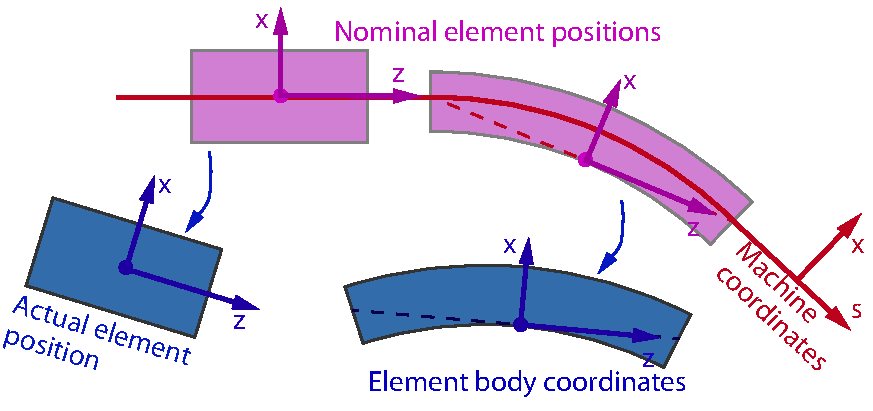
\includegraphics{alignment-ref.pdf} 
\caption[Element alignment.]  
{AlignmentGroup parameters The reference point is the origin
about which the element alignment is calculated. 
A) For straight elements, the reference point is in the center of the element. 
For \vn{Bend} elements, the reference point is at the midpoint of the chord connecting
the entrance point to the exit point.
}  \label{f:alignment}
\end{figure}

\begin{figure}
\centering 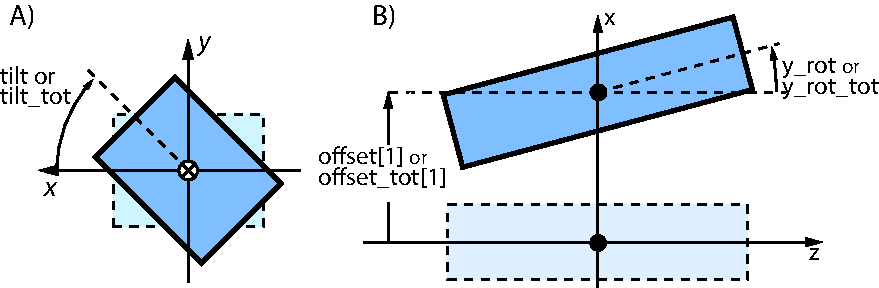
\includegraphics{alignment2.pdf} \caption[Alignment geometry.]  
{Alignment geometry. A) \vn{tilt} (or \vn{tilt_tot}) rotation. B) Combined
\vn{offset[1]} with \vn{y_rot} (or \vn{offset_tot[1]} with \vn{y_rot_tot}).
}  \label{f:alignment}
\end{figure}

The alignment group gives the alignment (position and angular orientation) of the physical element 
relative to the nominal position defined by the machine coordinates (\sref{s:orient}).
Alignment is specified with respect to the ``alignment reference point'' of an element as shown
in Fig~\ref{s:alignment}. 

The parameters of the \vn{AlignmentGroup} can be divided into two sub-groups. 
One group has a \vn{_tot} suffix:
\begin{example}
  offset_tot::Vector - $[x, y, z]$ offset.
  x_rot_tot::Number  - Rotation around the x-axis.
  y_rot_tot::Number  - Rotation around the z-axis.
  tilt_tot::Number   - Rotation around the z-axis. 
\end{example}
These ``total alignment'' parameters give the alignment of the element with 
with respect to the machine coordinates.
The other sub-group of parameters do not have a \vn{_tot} suffix:
\begin{example}
  offset::Vector - $[x, y, z]$ offset.
  x_rot::Number  - Rotation around the x-axis.
  y_rot::Number  - Rotation around the z-axis.
  tilt::Number   - Rotation around the z-axis. 
\end{example}
These ``relative alignment'' parameters give the alignment of the element with respect 
to any \vn{Girder} that is supporting the element. 
If there is no support \vn{Girder}, the total alignment will be the same as the relative
alignment. The relative alignment can be set by the User. 
The total alignment is computed by \accellat based upon the relative alignment and the alignment
of any \vn{Girder}. \vn{Girder} elements themselves also have both relative and total
alignments since Girders can support other Girders.


